\documentclass[conference]{IEEEtran}
\IEEEoverridecommandlockouts
\usepackage{booktabs}       % 修复 toprule midrule bottomrule
\usepackage{placeins}       % 修复 FloatBarrier
\usepackage{balance}
\usepackage{graphicx}
\usepackage{amsmath,amssymb,amsfonts}
\usepackage{algorithmic}
\usepackage{textcomp} 
\usepackage{xcolor}
\usepackage{cite}
%\usepackage{float}
%\usepackage[inkscapelatex=false]{svg} % 关键包
\graphicspath{{figs/}} % 图片放 figures 文件夹
\def\BibTeX{{\rm B\kern-.05em{\sc i\kern-.025em b}\kern-.08em
		T\kern-.1667em\lower.7ex\hbox{E}\kern-.125emX}}
\begin{document}
	
	% ===================== 标题 =====================
	\title{Target-Local Soft-Information Fusion for Communication-Constrained Multi-UAV OTFS-ISAC Sensing}
	
	% ===================== 作者（标准格式） =====================
	\author{
		\IEEEauthorblockN{
			Xinhang Tan,
			Zhengquan Zhang,
			L Hao
		}
		\IEEEauthorblockA{
			\textit{Southwest Jiaotong University}\\
			Chengdu, China\\
			Email: tanxinhang6478@163.com, zhang.zhengquan@swjtu.edu.cn, lhao@home.swjtu.edu.cn
		}
		\thanks{Corresponding author: Xinhang Tan.}
	}
	\maketitle
	
	% ===================== 摘要（纯净版） =====================

	\begin{abstract}
		Multi-UAV cooperative sensing gains depend not only on which observations are
		selected, but also on where their soft reports are fused. We propose a
		target-local fusion architecture for prior-assisted OTFS-ISAC sensing. Each
		target is assigned to the UAV nearest its predicted position; a communication-
		error-calibrated, adaptive coarse-to-fine (C2F) selector then screens and
		replays target-dependent sensing--reporting candidates using the implemented
		detector. The fusion rule uses predicted beliefs only and preserves the same
		finite-blocklength model, 640-bit packet, 2048 channel uses, and resource
		caps as the canonical system. In 1000 paired trials with 15 UAVs and 10
		targets, V1 attains $P_D=0.9762$ (95\% CI: $[0.9730,0.9790]$) and
		worst-target $P_D=0.967$. It selects 12.101 sensing observations but sends
		only 0.751 remote reports, corresponding to 0.481~kbit and 0.801~ms.
		Its paired gain over exact-marginal greedy is 0.0351, while its $P_D$ is
		statistically tied with sensing-SINR selection and uses 83.7\% less payload.
		A fusion-rule ablation and six operating-
		boundary sweeps show that the gain arises from target-related fusion planning
		jointly with two-stage selection, while large belief errors, strict rate
		thresholds, and sparse deployments remain the principal limitations.
	\end{abstract}

	\begin{IEEEkeywords}
		Multi-UAV networks, OTFS-ISAC, target-local fusion, cooperative sensing,
		finite-blocklength reporting, coarse-to-fine selection.
	\end{IEEEkeywords}


	\section{Introduction}
\label{sec:introduction}

Integrated sensing and communication (ISAC) allows a wireless network to reuse
spectrum, hardware, and signal-processing resources for transmission and
environmental sensing~\cite{liu_dual_functional_6g,gonzalez_revolution_2024}.
UAV-enabled ISAC further exploits mobility and favorable line-of-sight geometry
to extend sensing coverage~\cite{mu_uav_isac,meng_uav_isac_challenges}. When
multiple UAVs observe the same target from different bistatic geometries, their
soft decisions can provide complementary evidence~\cite{meng_cooperative_isac_2025}.

This cooperation is not free. Each observation is produced by a sensing chain
$i\!\rightarrow\!q\!\rightarrow\!j$ and must then be delivered from receiver
$j$ to a fusion UAV. A strong echo may contribute little if its reporting link
is unreliable, its delay--Doppler (DD) energy is poorly captured, or its packet
cost exceeds its marginal detection value~\cite{yuan_dd_isac,
keskin_mimo_otfs_isac,chen_node_selection_backhaul_2025}. Existing
node-selection and backhaul-aware studies address parts of this coupling, while
distributed-detection models often abstract away the bistatic geometry and
OTFS DD structure~\cite{chawla_massive_mimo_dd,
chawla_parameter_detection_mimo_wsn,meng_network_level_isac_2024}.

A further architectural choice has received less attention: \emph{where should
reports about each target meet?} A target-agnostic rule that maximizes a UAV's
aggregate incoming rate tends to assign every target to the same central
receiver. That concentration changes all reporting rates, finite-blocklength
success probabilities, and even the feasible candidate sets seen by the inner
selector. Thus, improving only the link-ranking formula cannot correct an
unfavorable fusion destination.

We study prior-assisted confirmation or re-detection and introduce target-local
fusion planning. For every target, the fusion UAV is chosen using the predicted
target position rather than the unknown truth. The resulting target-specific
reporting graph is passed to an adaptive two-stage C2F selector whose final
greedy replay is aligned with the implemented detector. This separation is
deliberate: the fusion rule changes the information available to the selector,
whereas the fair marginal-gain objective and resource constraints remain fixed.

Our main contributions are as follows.

\begin{itemize}
	\item We formulate joint target-specific fusion planning and triplet-level
	soft-report selection for multi-UAV bistatic OTFS-ISAC. The fusion destination
	depends only on the predicted target belief, preventing truth leakage into the
	scheduler.

	\item We combine this outer planning layer with communication-error calibration,
	an adaptive coarse frontier, waveform-derived DD refinement, and detector-aligned
	greedy replay. The inner fair utility and communication price are unchanged,
	which isolates the architectural role of fusion placement.

	\item We provide a reproducible V1 evaluation: a 1000-trial paired main
	comparison, a controlled fusion-rule ablation, reporting-structure diagnostics,
	and sweeps over belief error, rate threshold, deployment area, communication
	price, blocklength, and fleet size.

	\item We identify the operating boundary rather than reporting a single favorable
	point. The results distinguish measured serial latency from a prospective
	parallel-scheduling lower bound and distinguish confirmatory MC=1000 evidence
	from exploratory MC=100 sweeps.
\end{itemize}

The remainder of the paper presents the system model in
Section~\ref{sec:system_model}, the target-local C2F method in
Section~\ref{sec:proposed_algorithm}, the V1 evidence in
Section~\ref{sec:simulation_results}, and conclusions in
Section~\ref{sec:conclusion}.

	\section{System Model}
\label{sec:system_model}
\begin{figure}[t]
\centering
\resizebox{\linewidth}{!}{%
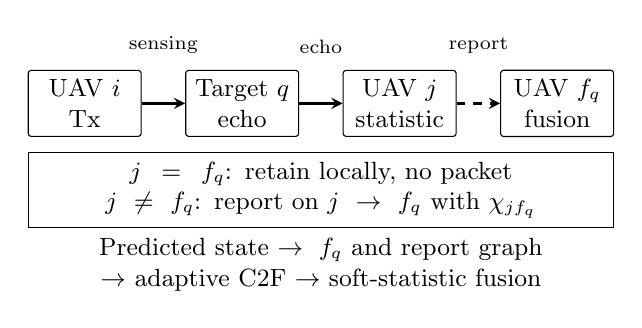
\begin{tikzpicture}[>=stealth, every node/.style={font=\small},
box/.style={draw,rounded corners=1pt,align=center,minimum height=8mm,text width=12mm}]
\node[box] (tx) at (0,0) {UAV $i$\\Tx};
\node[box] (tg) at (2,0) {Target $q$\\echo};
\node[box] (rx) at (4,0) {UAV $j$\\statistic};
\node[box] (fc) at (6,0) {UAV $f_q$\\fusion};
\draw[->,thick] (tx) -- node[above=5mm,font=\scriptsize] {sensing} (tg);
\draw[->,thick] (tg) -- node[above=5mm,font=\scriptsize] {echo} (rx);
\draw[->,thick,dashed] (rx) -- node[above=5mm,font=\scriptsize] {report} (fc);
\node[draw,align=center,text width=72mm] at (3,-1.1)
{$j=f_q$: retain locally, no packet\\
 $j\ne f_q$: report on $j\to f_q$ with $\chi_{jf_q}$};
\node[align=center,text width=72mm] at (3,-2.05)
{Predicted state $\to f_q$ and report graph\\
 $\to$ adaptive C2F $\to$ soft-statistic fusion};
\end{tikzpicture}}
\caption{Sensing and reporting have different endpoints. The fusion UAV is
chosen from predicted target state before observation selection and reporting.}
\label{fig:system_framework}
\end{figure}


\subsection{Task, Prior Information, and Reporting Graph}

Let $\mathcal M=\{1,\ldots,M\}$ and $\mathcal Q=\{1,\ldots,Q\}$ denote
UAVs and targets. Observation $e=(i,j,q)$ is generated at echo receiver $j$:
\begin{equation}
 i\rightarrow q\rightarrow j\rightarrow f_q .
 \label{eq:information_path}
\end{equation}
The sensing pair is $(i,j)$, whereas its reporting link is $(j,f_q)$.
All statistics for target $q$ meet at one fusion UAV $f_q$.
When $j=f_q$, no report is transmitted (Fig.~\ref{fig:system_framework}).

The task is confirmation or re-detection after upstream acquisition.
An external tracker supplies $b_q=\mathcal N(\widehat{\mathbf x}_q,\mathbf P_q)$;
we simulate its output with noisy horizontal position and velocity estimates,
keeping nominal target altitude known. Only this belief and the mean RCS
enter planning. The unknown current state enters echo generation and final
detection. The DD search gate propagates $\mathbf P_q$ through the bistatic
Jacobian and uses three standard deviations per DD coordinate. This gate
models search coverage, not a posterior tracker or blind initial acquisition.

\subsection{Reporting Reliability and Cost}

Sensing and reporting share power, $P_i^{\mathrm s}=\rho P_i$ and
$P_i^{\mathrm c}=(1-\rho)P_i$. The UAV channel gain is
$g_{ab}^{\mathrm c}=(\lambda/4\pi)^2d_{ab}^{-\alpha_{\mathrm c}}
\zeta_{ab}|h_{ab}^{\mathrm c}|^2$, with shadowing $\zeta_{ab}$ and fading
$h_{ab}^{\mathrm c}$. Under orthogonal serial reporting,
\begin{equation}
\begin{aligned}
 \gamma_{ab}^{\mathrm c}&=
 \frac{P_a^{\mathrm c}g_{ab}^{\mathrm c}}
 {N_0+\epsilon_{\mathrm s}\sum_{k\ne a,b}P_k^{\mathrm s}g_{kb}^{\mathrm c}
 +\epsilon_{\mathrm d}P_a^{\mathrm s}g_{ab}^{\mathrm c}},\\
 R_{ab}&=B_{\mathrm c}\log_2(1+\gamma_{ab}^{\mathrm c}).
\end{aligned}
 \label{eq:comm_sinr_rate}
\end{equation}
Here $N_0$ is receiver noise power over $B_{\mathrm c}$, and
$\epsilon_{\mathrm s},\epsilon_{\mathrm d}$ are residual sensing leakage factors.
Reports do not mutually interfere; sensing transmissions remain concurrent.

For a $k$-bit packet in $n$ channel uses, we adopt the normal approximation
for a complex AWGN-equivalent reporting channel~\cite{polyanskiy_fbl}:
\begin{equation}
 \chi_{ab}\simeq1-\mathsf Q\!\left(
 \frac{C(\gamma_{ab}^{\mathrm c})-k/n}
 {\sqrt{V(\gamma_{ab}^{\mathrm c})/n}}\right),
 \label{eq:fbl_reliability}
\end{equation}
where $C(\gamma)=\log_2(1+\gamma)$ and
$V(\gamma)=[1-(1+\gamma)^{-2}](\log_2 e)^2$.
This conditional packet-success approximation replaces the heuristic
$\gamma/(\gamma+\gamma_{\rm req})$; it is not a measured code-specific error curve.
A remote link must satisfy the range mask, $R_{ab}\ge R_{\min}$, and
$\chi_{ab}\ge\chi_{\min}$. Each selected remote observation reserves one
fixed padded $k$-bit report and $n/B_{\mathrm c}$ seconds, without aggregation
or retransmission. Thus $N_{\rm rem}$ reports cost $kN_{\rm rem}$ bits and
$nN_{\rm rem}/B_{\mathrm c}$ serial delay. Local delivery has $\chi=1$ and zero
reporting cost; sensing, processing, and unmodeled control traffic are not free.

\subsection{DD Energy and Local Statistic}

With $\mathbf u_{iq}$ pointing from UAV $i$ to target $q$, the bistatic
coordinates are
\begin{equation}
\begin{aligned}
 \tau_{ijq}&=(d_{iq}+d_{jq})/c,\\
 \nu_{ijq}&=\lambda^{-1}\!\left[(\mathbf v_q-\mathbf v_i)^T\mathbf u_{iq}
 +(\mathbf v_q-\mathbf v_j)^T\mathbf u_{jq}\right].
\end{aligned}
 \label{eq:bistatic_delay_doppler}
\end{equation}
Let $\ell=\tau L\Delta f$ and $\kappa=\nu NT$, with $T=1/\Delta f$.
The coarse estimate is $\eta^{\mathrm c}=\mathrm{sinc}^2(\ell-\mathrm{round}\ell)
\mathrm{sinc}^2(\kappa-\mathrm{round}\kappa)$.
For a periodic $A$-bin axis define
\begin{equation}
\begin{aligned}
 D_A(x)&=\frac{\sin(\pi x)}{A\sin(\pi x/A)},\quad
 p_A(b;z)=\frac{|D_A(b-z)|^2}{\sum_{a=0}^{A-1}|D_A(a-z)|^2},\\
 \eta^{\mathrm{loc}}_{ijq}
 &=\sum_{(b,d)\in\mathcal W_W(\kappa,\ell)}p_N(b;\kappa)p_L(d;\ell).
\end{aligned}
 \label{eq:local_dd_energy}
\end{equation}
The window contains $(2W+1)^2$ bins around the rounded center, with indices
wrapped modulo $(N,L)$. The removable singularity of $D_A$ is evaluated by
continuity. This normalized finite-grid leakage model gives
$0\le\eta^{\mathrm{loc}}\le1$. We use $W=1$ (nine bins) and
$\eta^{\mathrm f}=\eta^{\mathrm{loc}}$, with no interpolation coefficient or gain
floor. The fractional-center cache resolution is $10^{-3}$ bin.
The compact OTFS chain~\cite{hadani_otfs} is checked separately below;
$W=1$ is a fixed processing choice, not a proved optimal window.

With mean target RCS $\bar\sigma_q$,
$g_{ijq}^{\mathrm s}=\lambda^2\bar\sigma_q/[(4\pi)^3d_{iq}^2d_{jq}^2]$,
and
\begin{equation}
 \gamma_{ijq}^{\mathrm s}=
 \frac{P_i^{\mathrm s}g_{ijq}^{\mathrm s}G_{ij}^{\mathrm{hw}}G_{\mathrm p}
 \eta_{ijq}^{\mathrm{DD}}\eta_{ijq}^{\mathrm{col}}}
 {N_0+I_j^{\mathrm s}}.
 \label{eq:sensing_sinr}
\end{equation}
Here $G_{ij}^{\mathrm{hw}}$ contains antenna gains and losses, and $I_j^{\mathrm s}$
includes residual self-interference and concurrent direct paths.
The collision surrogate is $\eta^{\mathrm{col}}=1/n_{ijq}$, where $n_{ijq}$
counts targets in the same rounded DD bin for pair $(i,j)$.
It is an occupancy penalty, not a coherent multi-target interference law.

For $K_{\rm look}$ independent looks, normalized energy $X$ has Gamma shape
$K_{\rm look}$ and scale $1$ under $\mathcal H_0$, or $1+\gamma$ under
$\mathcal H_1$. The centered LLR is
\begin{equation}
 \ell_e=\frac{\gamma}{1+\gamma}(X-K_{\rm look}).
 \label{eq:local_llr}
\end{equation}
Consequently, $\delta_e=K_{\rm look}\gamma^2/(1+\gamma)$,
$v_{e,0}=K_{\rm look}\gamma^2/(1+\gamma)^2$, and
$v_{e,1}=K_{\rm look}\gamma^2$. Look-to-look fluctuation is marginalized by
this energy law rather than sampled again in the mean-RCS link budget.

For successful delivery $A_e\sim\mathrm{Bernoulli}(\chi_e)$, set
$Y_e=A_e\ell_e+(1-A_e)Z_e$, with independent
$Z_e\sim\mathcal N(0,a v_{e,0})$. Total expectation and variance give
\begin{equation}
\begin{aligned}
 \delta_e^{\rm eff}&=\chi_e\delta_e,\\
 \bar v_{e,0}&=[\chi_e+(1-\chi_e)a]v_{e,0},\\
 \bar v_{e,1}&=\chi_ev_{e,1}+(1-\chi_e)av_{e,0}
 +\chi_e(1-\chi_e)\delta_e^2.
\end{aligned}
 \label{eq:received_moments}
\end{equation}
The archived V1 implementation uses $a=9$: failed reports are replaced by
zero-mean uncertainty. This Gaussian replacement is an explicit surrogate,
not a consequence of finite blocklength or a true erasure ($a=0$).
The between-component term in $\bar v_{e,1}$ cannot be omitted.

For independent selected observations, use
$w_e\propto\delta_e^{\rm eff}/\bar v_{e,0}$,
$m_{q,1}=\sum_{e\in\mathcal S_q}w_e\delta_e^{\rm eff}$, and
$v_{q,h}=\sum_{e\in\mathcal S_q}w_e^2\bar v_{e,h}$. The selector predicts
\begin{equation}
\begin{aligned}
 t_q&=\sqrt{v_{q,0}}\left[z_0+\frac{\kappa_{q,0}}6(z_0^2-1)\right],\\
 \widehat P_{D,q}&=\mathsf Q\!\left(\frac{t_q-m_{q,1}}{\sqrt{v_{q,1}}}\right),
\end{aligned}
 \label{eq:detector_prediction}
\end{equation}
where $z_0=\mathsf Q^{-1}(P_{\mathrm{FA}})$ and $\kappa_{q,0}$ is null skewness.
Empty-set prediction is zero. Scheduling uses belief-based moments; final
Monte Carlo detection uses truth-side observations and the same threshold
rule. This remains a moment approximation, not an exact detection probability.
The supplement documents the archived failure-model naming and validation.

	\section{Target-Local Adaptive C2F Selection}
\label{sec:proposed_algorithm}

\subsection{Prediction-Only Fusion Placement}

The outer stage assigns each target to the UAV nearest its predicted position:
\begin{equation}
	f_q=\arg\min_{m\in\mathcal M}
	\|\widehat{\mathbf p}_q-\mathbf p_m^{\mathrm{UAV}}\|_2 .
	\label{eq:nearest_target_fusion}
\end{equation}
The rule uses neither the current target truth nor its realized RCS. It is a
low-complexity placement heuristic, not a jointly optimal fusion solution.
Given $f_q$, the feasible observation set is
\begin{equation}
\begin{aligned}
	\mathcal E_q=\{(i,j,q):{}&(i,j,q)\text{ is DD-valid},\\
	&j=f_q\text{ or }(j,f_q)\text{ is feasible}\}.
\end{aligned}
	\label{eq:feasible_candidate_set}
\end{equation}

\noindent\textit{Local-delivery bound.}
Under \eqref{eq:received_moments}, the single-observation deflection is
$d(\chi)=\chi^2\delta^2/[v_0(a+(1-a)\chi)]$. Its derivative is nonnegative
for $a\ge0$, so local delivery maximizes this quantity for the same observation.
This does not imply monotonicity of the approximate $P_D$ or optimality of
nearest-target placement when other report links change.

For fixed observation laws and hypothesis-independent replacement, lower
reliability is a random degradation of higher reliability. Optimal detection
at fixed false alarm is therefore nondecreasing with reliability
~\cite{blackwell_experiments}. The supplementary proof concerns the optimal
ROC envelope, not the implemented linear detector.

For a fixed $\mathcal S_q$, let $a_{qm}$ count selected observations received
at UAV $m$. Every fusion choice obeys
$N_{{\rm rem},q}\ge |\mathcal S_q|-\max_m a_{qm}$.
This follows because only observations produced at the fusion UAV avoid a
packet. A feasible nearest-target assignment attaining the bound is
report-minimal for that fixed set; no joint selection optimum is implied.

\subsection{Communication-Constrained Selection}

Let $\widehat{\mathbf P}_D(\mathcal S)$ denote the detector-predicted target
probabilities from \eqref{eq:detector_prediction}. We cap each target probability
at the design requirement and define a smooth weak-target utility
\begin{equation}
\begin{aligned}
	U(\widehat{\mathbf P}_D)=&-Q\tau_\alpha\log\sum_q
	\exp[-\bar P_{D,q}/\tau_\alpha]\\
	&-\frac{\mu_\alpha}{2P_D^{\rm req}}
	\sum_q[P_D^{\rm req}-\widehat P_{D,q}]_+^2,
\end{aligned}
	\label{eq:fair_sensing_utility}
\end{equation}
where $\bar P_{D,q}=\min(\widehat P_{D,q},P_D^{\rm req})$. The first term
prioritizes weak targets, while the second penalizes unresolved detection gaps.
The selector heuristically seeks a high value of the capped objective:
\begin{equation}
\begin{aligned}
	\max_{\mathcal S\subseteq\cup_q\mathcal E_q}\quad
	&F(\mathcal S)=U(\widehat{\mathbf P}_D(\mathcal S))
	-\lambda_c\sum_{e\in\mathcal S}c_e,\\
	\mathrm{s.t.}\quad&|\mathcal S_q|\le L_{\max},\quad
	|\mathcal S|\le L_{\mathrm{tot}},
\end{aligned}
	\label{eq:task_objective}
\end{equation}
where $c_e=10^3\mathbf1\{j\ne f_q\}n/B_{\mathrm c}$ is measured in
milliseconds, matching the implemented price $\lambda_c$. Fixed blocklength makes
$c_e$ a remote-report cardinality price rather than a link-dependent delay.
The caps limit observations, including local ones; the price does not enforce
a prescribed hard communication budget. They imply payload at most
$kL_{\rm tot}$ and serial delay at most $nL_{\rm tot}/B_{\rm c}$.
The greedy replay repeatedly commits the feasible candidate with the largest
positive marginal $F(\mathcal S\cup\{e\})-F(\mathcal S)$. Because the objective
can be non-monotone and the constraints combine target and total caps, we claim
neither global optimality nor a universal submodular approximation ratio.

\subsection{Adaptive C2F Acceleration}
\begin{table}[t]
\caption{Prediction-only adaptive C2F (released V1)}
\label{alg:adaptive_c2f}
\footnotesize
\begin{algorithmic}[1]
\REQUIRE Belief-side tables, $f_q$, caps, $J=25$, $W=1$
\STATE Build triplet sets $\mathcal E_q$; set $S=\varnothing$, $H_q=\varnothing$.
\WHILE{$|S|<L_{\rm tot}$}
\STATE Compute coarse $\Delta F(e\mid S)$ for unselected candidates
satisfying caps and $\Delta D_q>0$.
\STATE For each target, add its highest positive-gain candidate outside
$H_q$ if $|H_q|<\min(J,|\mathcal E_q|)$.
\STATE Let $e^*$ have largest positive gain; stop if none exists.
\STATE Commit $e^*$ to $S$. Insert it into $H_q$ if absent,
replacing the last entry when full.
\ENDWHILE
\STATE Evaluate $\eta^{\rm loc}$ only on $H=\bigcup_q H_q$.
\STATE Reset $S=\varnothing$; greedily add the largest positive fine
$\Delta F$ on $H$, checking caps and $\Delta D_q>0$ each time.
\RETURN $S$ when no admissible positive gain remains or the total cap binds.
\end{algorithmic}
\end{table}


The pseudocode in Table~\ref{alg:adaptive_c2f} constructs a per-target frontier,
then replays the same objective on its fine estimates. The per-target
shortlist cap is $J=25$ and the observation cap is six. A positive-deflection
filter uses $D_q=\sum_{e\in S_q}d(\chi_e)$ under independence.
Cached moments are invalidated when their target's selected set changes.
Ties retain the first candidate in target/transmitter/receiver order.

Let $E$ be the number of feasible candidates and $r$ the number refined. If a
coarse evaluation costs $C_{\mathrm c}$ and a fine evaluation costs
$C_{\mathrm f}$, full refinement costs $EC_{\mathrm f}$, whereas adaptive C2F
has DD evaluation cost approximately
\begin{equation}
	EC_{\mathrm c}+rC_{\mathrm f},\qquad r\le E.
	\label{eq:c2f_complexity}
\end{equation}
This excludes greedy scoring and frontier maintenance. With at most
$L_{\mathrm{tot}}$ commits per stage, scanning requires
$O(L_{\mathrm{tot}}(E+r))$ candidate-score evaluations; a direct implementation costs
$O(L_{\rm tot}(E+r)(L_{\max}+Q))$ for moments and global utility evaluation,
before caching. Nearest placement costs $O(QM)$ and the shortlist stores
at most $QJ$ triplets. When fine DD refinement dominates, the fractional reduction approaches $1-r/E$.
The main experiment used 61.3 refinements for 860.2 feasible candidates
(92.9\% fewer). This is a work-count ratio, not a wall-clock speedup.
No bound on omitted candidates is available, so C2F is not claimed lossless.
  % 已修复无空格
	\section{Simulation Results}
\label{sec:simulation_results}

\begin{figure*}[!t]
	\centering
	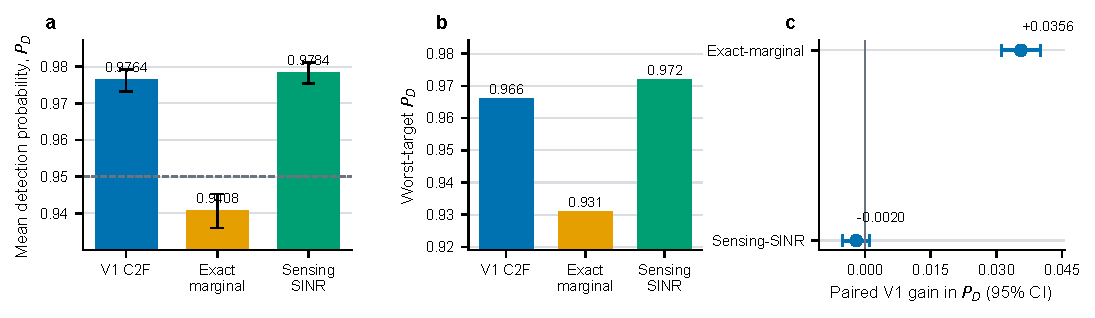
\includegraphics[width=0.98\textwidth]{figs/fig2_v1_main_comparison.pdf}
	\caption{Confirmatory MC=1000 comparison under identical per-trial resources.
	(a) Mean detection probability with 95\% Wilson intervals; the dashed line
	marks 0.95. (b) Worst-target detection probability. (c) Paired V1-minus-
	baseline differences with 95\% confidence intervals.}
	\label{fig:v1_main}
\end{figure*}

\begin{figure*}[!t]
	\centering
	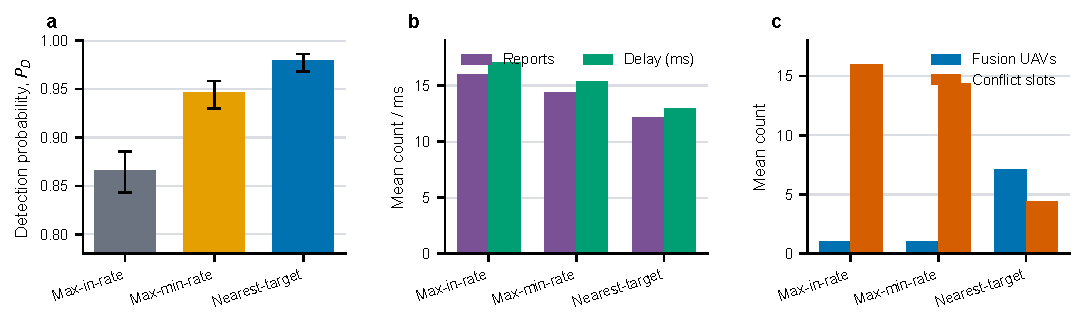
\includegraphics[width=0.98\textwidth]{figs/fig3_v1_fusion_ablation.pdf}
	\caption{Fusion-rule mechanism ablation (MC=100 per rule) with the inner
	adaptive C2F selector fixed. (a) Detection probability and 95\% intervals.
	(b) Selected reports and measured serial delay. (c) Number of assigned fusion
	UAVs and conflict-graph slots. The slot count diagnoses parallelization
	potential; it is not an achieved latency.}
	\label{fig:fusion_ablation}
\end{figure*}

\begin{figure*}[!t]
	\centering
	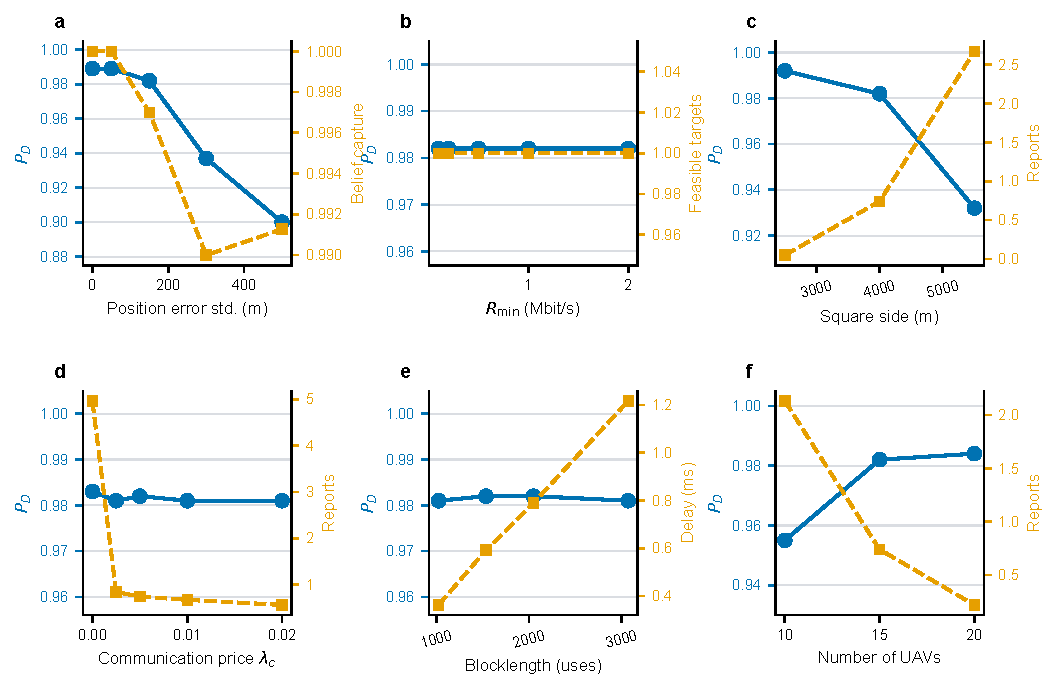
\includegraphics[width=0.98\textwidth]{figs/fig4_v1_operating_envelope.pdf}
	\caption{Exploratory V1 operating envelope (MC=100 per condition). Blue circles
	show $P_D$; orange squares show the named secondary metric. (a) Position-belief
	error, (b) minimum reporting rate, (c) deployment side length, (d)
	communication price, (e) blocklength, and (f) UAV fleet size.}
	\label{fig:operating_envelope}
\end{figure*}

\subsection{Protocol and Nominal Configuration}

We evaluate prior-assisted confirmation in a $4000\,\mathrm{m}\times
4000\,\mathrm{m}$ region with $M=15$ UAVs and $Q=10$ targets. Table~
\ref{tab:simulation_parameters} lists the released V1 configuration. All main
methods use the same paired geometries, detector randomness, feasible graph,
and per-trial number of selected reports. The confirmatory comparison uses 1000
Monte-Carlo trials. Fusion and operating-envelope sweeps use 100 trials per
condition with seed 2026 and are therefore diagnostic rather than substitutes
for the main evidence.

\begin{table}[!t]
	\centering
	\caption{Target-local fusion V1 simulation parameters}
	\label{tab:simulation_parameters}
	\footnotesize
	\setlength{\tabcolsep}{3pt}
	\begin{tabular}{@{}p{0.43\linewidth}p{0.51\linewidth}@{}}
		\toprule
		Parameter & Value \\
		\midrule
		UAVs / targets & $M=15$, $Q=10$ \\
		Area / communication range & $4000^2~\mathrm{m}^2$, $d_{\max}=2500~\mathrm m$ \\
		UAV / target speed & $30$--$60$ / $50$--$90~\mathrm{m/s}$ \\
		Carrier / DD grid & $5.9~\mathrm{GHz}$, $N=L=64$, $\Delta f=30~\mathrm{kHz}$ \\
		Power split / transmit power & $\rho=0.8$, $P_i=1~\mathrm W$ \\
		Rate threshold / false alarm & $R_{\min}=0.2~\mathrm{Mbit/s}$, $P_{\mathrm{FA}}=0.05$ \\
		Report / blocklength & 640 bits, $n=2048$ channel uses \\
		Predicted belief & $\sigma_p=150~\mathrm m$, $\sigma_v=15~\mathrm{m/s}$ \\
		Selection & $D_{\min}=3$, $\lambda_c=0.005$, $L_{\max}=6$, $L_{\mathrm{tot}}=60$ \\
		Fusion / reporting & nearest predicted target / serial orthogonal MAC \\
		C2F refinement & $W=1$, adaptive frontier, detector-aligned replay \\
		Main / sweep trials & 1000 / 100 per condition \\
		\bottomrule
	\end{tabular}
\end{table}

\subsection{Confirmatory Main Comparison}

Figure~\ref{fig:v1_main} compares target-local adaptive C2F with two strong
resource-matched rules. Exact-marginal greedy uses the same fair utility but no
C2F detector-aligned replay; Sensing-SINR ranks nominal sensing strength. V1
attains $P_D=0.9734$ (95\% CI: $[0.9701,0.9764]$), versus 0.9667 for
exact-marginal greedy and 0.9649 for Sensing-SINR. Its worst-target detection
probability is 0.968, compared with 0.957 and 0.953. The paired gains are
$+0.0067$ (95\% CI: $[0.0041,0.0093]$) and $+0.0085$
($[0.0061,0.0109]$), respectively; both interval lower bounds are positive.
The empirical active-target and system-wide false-alarm probabilities are
0.0498 and 0.0495, consistent with the designed value 0.05.

Resource matching is exact: each method selects 11.993 reports on average,
corresponding to 7.676~kbit and 12.793~ms of serial reporting. Thus, the main
detection gain is not purchased with more reports. The adaptive C2F stage
evaluates 117.7 fine DD neighborhoods instead of 509.3 for exhaustive local
refinement, reducing fine evaluations by 76.9\%. These results support the V1
system as a stable nominal point; they do not isolate fusion placement because
all three main methods already use the target-local graph.

\subsection{Why Target-Local Fusion Helps}

Figure~\ref{fig:fusion_ablation} changes only the fusion destination rule. The
target-agnostic max-in-rate rule gives $P_D=0.866$, worst-target $P_D=0.800$,
15.99 reports, and 17.056~ms. A max-min-rate alternative improves these values
to 0.946, 0.930, 14.36, and 15.317~ms. Nearest-target fusion reaches 0.979 and
0.960 with only 12.16 reports and 12.971~ms. Because the two-stage screening,
greedy objective, packets, and caps are unchanged, this ablation supports the
mechanism in \eqref{eq:nearest_target_fusion}: fusion placement changes the
reliable reporting-edge set seen by the selector.

The reporting structure explains the difference. Max-in-rate and max-min-rate
assign all ten targets to one fusion UAV on average. Nearest-target assigns
them across 7.13 UAVs and lowers the mean conflict-graph requirement from
15.99/14.36 to 4.40 slots. If reports in nonconflicting edges could be sent
simultaneously without bandwidth sharing, additional interference, or a changed
finite-blocklength model, 4.40 slots would correspond to a 4.693~ms lower
bound. V1 does not implement this scheduler, so its reported latency remains
the measured serial value 12.971~ms.

\subsection{Operating Envelope and Design Choices}

Figure~\ref{fig:operating_envelope} summarizes six controlled scans. First,
V1 remains near $P_D=0.98$ for position-error standard deviations up to 150~m,
then decreases to 0.960 at 300~m and 0.918 at 500~m. Belief capture remains
0.9868 even at 500~m; the degradation is therefore more consistent with
prediction-induced fusion and link mismatch than with DD-gate misses alone.
Second, $R_{\min}\le0.5$~Mbit/s is inactive at this nominal geometry. At
2~Mbit/s, only 94\% of targets retain feasible candidates and $P_D$ falls to
0.901; the lower report count is candidate starvation, not improved efficiency.

Topology is the next boundary. Increasing the square side from 2500 to 5500~m
changes $P_D$ from 0.992 to 0.913 and reports from 10.19 to 15.87. Increasing
the fleet from 10 to 20 UAVs at $Q=10$ changes $P_D$ from 0.941 to 0.987 while
reducing reports from 15.01 to 10.94. These scans vary density implicitly and
must not be combined into an independent density effect.

The communication price exhibits a broad plateau. Setting $\lambda_c=0$
requires 16.29 reports at $P_D=0.978$, whereas $\lambda_c=0.005$ uses 12.16
reports at $P_D=0.979$. Values from 0.0025 to 0.01 have overlapping MC=100
uncertainty, so 0.005 is treated as a stable engineering point rather than a
statistically unique optimum. Finally, 2048 channel uses yields
$P_D=0.979$ and 12.971~ms. The 1536-use setting is a promising lower-latency
candidate (0.977, 9.880~ms), while 3072 uses is dominated in this scan (0.975,
19.136~ms). A paired high-MC comparison is required before promoting the
1536-use setting to a new release.

All figures are generated directly from the released CSV/JSON records. The
resolved V1 configuration, source-data index, and plotting command accompany
the manuscript, preventing exploratory and confirmatory results from being
silently mixed.

	
	\balance
	\section{Conclusion}
\label{sec:conclusion}

This paper presented target-local fusion V1 for prior-assisted multi-UAV
OTFS-ISAC sensing. The outer planner assigns each target to the UAV nearest its
predicted position, while the existing communication-calibrated adaptive C2F
selector performs detector-aligned greedy replay. The formulation therefore
changes where reports meet while the detector-PD objective independently
chooses its observation set under fixed packet, blocklength, and resource caps.

In 1000 paired trials, V1 achieved $P_D=0.9762$ and worst-target
$P_D=0.967$ from 12.101 observations, with only 0.751 remote reports,
0.481~kbit, and 0.801~ms of serial reporting. Its paired gain over
exact-marginal greedy was 0.0351. Its detection rate was statistically tied
with Sensing-SINR, while using 83.7\% less payload. A controlled fusion-rule
ablation showed that target-local planning disperses targets across fusion UAVs
and exposes shorter, more reliable reporting edges to the inner selector. The
evidence therefore supports a combined architectural conclusion: target-related
fusion planning plus adaptive two-stage selection---rather than attributing the
full improvement to a new greedy criterion.

V1 is a stable nominal version, not a universal endpoint. Large prediction
errors and sparse deployments remain its principal boundaries. The present
rate-threshold scan is weak because local evidence dominates remote reporting.
Future work will add fusion capacity and sensing-acquisition costs, validate the
analytic DD proxy at waveform level, model obstruction and correlated reports,
and optimize link-dependent blocklengths instead of a fixed report price.

	% ===================== 参考文献（IEEE 标准格式） =====================
	%
%\begin{thebibliography}{00}
%	
%	\bibitem{liu_isac_survey}
%	A. Liu, Z. Huang, M. Li, Y. Wan, W. Li, T. X. Han, C. Liu, R. Du,
%	D. K. P. Tan, J. Lu, Y. Shen, F. Colone, and K. Chetty,
%	``A survey on fundamental limits of integrated sensing and communication,''
%	\emph{IEEE Communications Surveys \& Tutorials}, vol. 24, no. 2,
%	pp. 994--1034, 2022.
%	
%	\bibitem{liu_dual_functional_6g}
%	F. Liu, Y. Cui, C. Masouros, J. Xu, T. X. Han, Y. C. Eldar, and S. Buzzi,
%	``Integrated sensing and communications: Toward dual-functional wireless
%	networks for 6G and beyond,''
%	\emph{IEEE Journal on Selected Areas in Communications}, vol. 40, no. 6,
%	pp. 1728--1767, Jun. 2022.
%	
%	\bibitem{gonzalez_revolution_2024}
%	N. Gonzalez-Prelcic, M. F. Keskin, O. Kaltiokallio, M. Valkama,
%	D. Dardari, X. Shen, Y. Shen, M. Bayraktar, and H. Wymeersch,
%	``The integrated sensing and communication revolution for 6G: Vision,
%	techniques, and applications,''
%	\emph{Proceedings of the IEEE}, vol. 112, no. 7,
%	pp. 676--723, Jul. 2024.
%	
%	\bibitem{kaushik_6g_standardization_2024}
%	A. Kaushik, R. Singh, S. Dayarathna, R. Senanayake, M. Di Renzo,
%	M. Dajer, H. Ji, Y. Kim, V. Sciancalepore, A. Zappone, and W. Shin,
%	``Toward integrated sensing and communications for 6G: Key enabling technologies,
%	standardization, and challenges,''
%	\emph{IEEE Communications Standards Magazine}, vol. 8, no. 2,
%	pp. 52--59, Jun. 2024.
%	
%	\bibitem{meng_cooperative_isac_2025}
%	K. Meng, C. Masouros, A. P. Petropulu, and L. Hanzo,
%	``Cooperative ISAC networks: Performance analysis, scaling laws, and optimization,''
%	\emph{IEEE Transactions on Wireless Communications}, vol. 24, no. 2,
%	pp. 877--892, Feb. 2025.
%	
%	\bibitem{meng_network_level_isac_2024}
%	K. Meng, C. Masouros, G. Chen, and F. Liu,
%	``Network-level integrated sensing and communication: Interference management
%	and BS coordination using stochastic geometry,''
%	\emph{IEEE Transactions on Wireless Communications}, vol. 23, no. 12,
%	pp. 19365--19381, Dec. 2024.
%	
%	\bibitem{mu_uav_isac}
%	J. Mu, R. Zhang, Y. Cui, N. Gao, and X. Jing,
%	``UAV meets integrated sensing and communication: Challenges and future directions,''
%	\emph{IEEE Communications Magazine}, vol. 61, no. 5,
%	pp. 62--67, May 2023.
%	
%	\bibitem{meng_uav_isac_challenges}
%	K. Meng, Q. Wu, J. Xu, W. Chen, Z. Feng, R. Schober, and A. L. Swindlehurst,
%	``UAV-enabled integrated sensing and communication: Opportunities and challenges,''
%	\emph{IEEE Wireless Communications}, vol. 31, no. 2,
%	pp. 97--104, Apr. 2024.
%	
%	\bibitem{khuwaja_uav_channel_survey}
%	A. A. Khuwaja, Y. Chen, N. Zhao, M.-S. Alouini, and P. Dobbins,
%	``A survey of channel modeling for UAV communications,''
%	\emph{IEEE Communications Surveys \& Tutorials}, vol. 20, no. 4,
%	pp. 2804--2821, Fourthquarter 2018.
%	
%	\bibitem{chawla_massive_mimo_dd}
%	A. Chawla, A. Patel, A. K. Jagannatham, and P. K. Varshney,
%	``Distributed detection in massive MIMO wireless sensor networks under perfect and imperfect CSI,''
%	\emph{IEEE Transactions on Signal Processing}, vol. 67, no. 15,
%	pp. 4055--4068, Aug. 2019.
%	
%	\bibitem{chawla_parameter_detection_mimo_wsn}
%	A. Chawla, A. S. Sarode, A. K. Jagannatham, and L. Hanzo,
%	``Distributed parameter detection in massive MIMO wireless sensor networks relying on imperfect CSI,''
%	\emph{IEEE Transactions on Wireless Communications}, vol. 20, no. 1,
%	pp. 506--519, Jan. 2021.
%	
%	\bibitem{chen_node_selection_backhaul_2025}
%	M. Chen, M.-M. Zhao, A. Liu, M. Li, and Q. Shi,
%	``Joint node selection and resource allocation optimization for cooperative sensing with a shared wireless backhaul,''
%	\emph{IEEE Transactions on Signal Processing}, vol. 73,
%	pp. 67--82, 2025.
%	
%	\bibitem{hadani_otfs}
%	R. Hadani, S. Rakib, M. Tsatsanis, A. Monk, A. J. Goldsmith,
%	A. F. Molisch, and R. Calderbank,
%	``Orthogonal time frequency space modulation,''
%	in \emph{Proc. IEEE Wireless Communications and Networking Conference (WCNC)},
%	San Francisco, CA, USA, Mar. 2017, pp. 1--6.
%	
%	\bibitem{yuan_dd_isac}
%	W. Yuan, L. Zhou, S. K. Dehkordi, S. Li, P. Fan, G. Caire, H. V. Poor, and X. Wang,
%	``From OTFS to DD-ISAC: Integrating sensing and communications in the delay Doppler domain,''
%	\emph{IEEE Wireless Communications}, vol. 31, no. 6,
%	pp. 152--160, Dec. 2024.
%	
%	\bibitem{keskin_mimo_otfs_isac}
%	M. F. Keskin, C. Marcus, O. Eriksson, A. Alvarado, J. Widmer, and H. Wymeersch,
%	``Integrated sensing and communications with MIMO-OTFS: ISI/ICI exploitation and delay-Doppler multiplexing,''
%	\emph{IEEE Transactions on Wireless Communications}, vol. 23, no. 8,
%	pp. 10229--10246, Aug. 2024.
%	
%\end{thebibliography}
%
%\begin{thebibliography}{00}
%	
%	\bibitem{liu_dual_functional_6g}
%	F. Liu, Y. Cui, C. Masouros, J. Xu, T. X. Han, Y. C. Eldar, and S. Buzzi,
%	``Integrated sensing and communications: Toward dual-functional wireless networks for 6G and beyond,''
%	\emph{IEEE Journal on Selected Areas in Communications}, vol. 40, no. 6,
%	pp. 1728--1767, Jun. 2022.
%	
%	\bibitem{gonzalez_revolution_2024}
%	N. Gonzalez-Prelcic, M. F. Keskin, O. Kaltiokallio, M. Valkama,
%	D. Dardari, X. Shen, Y. Shen, M. Bayraktar, and H. Wymeersch,
%	``The integrated sensing and communication revolution for 6G: Vision, techniques, and applications,''
%	\emph{Proceedings of the IEEE}, vol. 112, no. 7,
%	pp. 676--723, Jul. 2024.
%	
%	\bibitem{meng_cooperative_isac_2025}
%	K. Meng, C. Masouros, A. P. Petropulu, and L. Hanzo,
%	``Cooperative ISAC networks: Performance analysis, scaling laws, and optimization,''
%	\emph{IEEE Transactions on Wireless Communications}, vol. 24, no. 2,
%	pp. 877--892, Feb. 2025.
%	
%	\bibitem{meng_network_level_isac_2024}
%	K. Meng, C. Masouros, G. Chen, and F. Liu,
%	``Network-level integrated sensing and communication: Interference management
%	and BS coordination using stochastic geometry,''
%	\emph{IEEE Transactions on Wireless Communications}, vol. 23, no. 12,
%	pp. 19365--19381, Dec. 2024.
%	
%	\bibitem{mu_uav_isac}
%	J. Mu, R. Zhang, Y. Cui, N. Gao, and X. Jing,
%	``UAV meets integrated sensing and communication: Challenges and future directions,''
%	\emph{IEEE Communications Magazine}, vol. 61, no. 5,
%	pp. 62--67, May 2023.
%	
%	\bibitem{meng_uav_isac_challenges}
%	K. Meng, Q. Wu, J. Xu, W. Chen, Z. Feng, R. Schober, and A. L. Swindlehurst,
%	``UAV-enabled integrated sensing and communication: Opportunities and challenges,''
%	\emph{IEEE Wireless Communications}, vol. 31, no. 2,
%	pp. 97--104, Apr. 2024.
%	
%	\bibitem{chawla_massive_mimo_dd}
%	A. Chawla, A. Patel, A. K. Jagannatham, and P. K. Varshney,
%	``Distributed detection in massive MIMO wireless sensor networks under perfect and imperfect CSI,''
%	\emph{IEEE Transactions on Signal Processing}, vol. 67, no. 15,
%	pp. 4055--4068, Aug. 2019.
%	
%	\bibitem{chawla_parameter_detection_mimo_wsn}
%	A. Chawla, A. S. Sarode, A. K. Jagannatham, and L. Hanzo,
%	``Distributed parameter detection in massive MIMO wireless sensor networks relying on imperfect CSI,''
%	\emph{IEEE Transactions on Wireless Communications}, vol. 20, no. 1,
%	pp. 506--519, Jan. 2021.
%	
%	\bibitem{chen_node_selection_backhaul_2025}
%	M. Chen, M.-M. Zhao, A. Liu, M. Li, and Q. Shi,
%	``Joint node selection and resource allocation optimization for cooperative sensing with a shared wireless backhaul,''
%	\emph{IEEE Transactions on Signal Processing}, vol. 73,
%	pp. 67--82, 2025.
%	
%	\bibitem{yuan_dd_isac}
%	W. Yuan, L. Zhou, S. K. Dehkordi, S. Li, P. Fan, G. Caire, H. V. Poor, and X. Wang,
%	``From OTFS to DD-ISAC: Integrating sensing and communications in the delay Doppler domain,''
%	\emph{IEEE Wireless Communications}, vol. 31, no. 6,
%	pp. 152--160, Dec. 2024.
%	
%	\bibitem{keskin_mimo_otfs_isac}
%	M. F. Keskin, C. Marcus, O. Eriksson, A. Alvarado, J. Widmer, and H. Wymeersch,
%	``Integrated sensing and communications with MIMO-OTFS: ISI/ICI exploitation and delay-Doppler multiplexing,''
%	\emph{IEEE Transactions on Wireless Communications}, vol. 23, no. 8,
%	pp. 10229--10246, Aug. 2024.
%	
%\end{thebibliography}

\begin{thebibliography}{00}
	
	\bibitem{liu_dual_functional_6g}
	F. Liu \emph{et al.}, ``Integrated sensing and communications: Toward dual-functional wireless networks for 6G and beyond,'' \emph{IEEE J. Sel. Areas Commun.}, vol. 40, no. 6, pp. 1728--1767, Jun. 2022, doi: 10.1109/JSAC.2022.3156632.
	
	\bibitem{gonzalez_revolution_2024}
	N. Gonz'alez-Prelcic \emph{et al.}, ``The integrated sensing and communication revolution for 6G: Vision, techniques, and applications,'' \emph{Proc. IEEE}, vol. 112, no. 7, pp. 676--723, Jul. 2024, doi: 10.1109/JPROC.2024.3397609.
	
	\bibitem{meng_cooperative_isac_2025}
	K. Meng, C. Masouros, A. P. Petropulu, and L. Hanzo, ``Cooperative ISAC networks: Performance analysis, scaling laws, and optimization,'' \emph{IEEE Trans. Wireless Commun.}, vol. 24, no. 2, pp. 877--892, Feb. 2025, doi: 10.1109/TWC.2024.3491356.
	
	\bibitem{meng_network_level_isac_2024}
	K. Meng, C. Masouros, G. Chen, and F. Liu, ``Network-level integrated sensing and communication: Interference management and BS coordination using stochastic geometry,'' \emph{IEEE Trans. Wireless Commun.}, vol. 23, no. 12, pp. 19365--19381, Dec. 2024, doi: 10.1109/TWC.2024.3483031.
	
	\bibitem{mu_uav_isac}
	J. Mu, R. Zhang, Y. Cui, N. Gao, and X. Jing, ``UAV meets integrated sensing and communication: Challenges and future directions,'' \emph{IEEE Commun. Mag.}, vol. 61, no. 5, pp. 62--67, May 2023, doi: 10.1109/MCOM.008.2200510.
	
	\bibitem{meng_uav_isac_challenges}
	K. Meng \emph{et al.}, ``UAV-enabled integrated sensing and communication: Opportunities and challenges,'' \emph{IEEE Wireless Commun.}, vol. 31, no. 2, pp. 97--104, Apr. 2024, doi: 10.1109/MWC.131.2200442.
	
	\bibitem{chawla_massive_mimo_dd}
	A. Chawla, A. Patel, A. K. Jagannatham, and P. K. Varshney, ``Distributed detection in massive MIMO wireless sensor networks under perfect and imperfect CSI,'' \emph{IEEE Trans. Signal Process.}, vol. 67, no. 15, pp. 4055--4068, Aug. 2019, doi: 10.1109/TSP.2019.2924588.
	
	\bibitem{chawla_parameter_detection_mimo_wsn}
	A. Chawla, A. S. Sarode, A. K. Jagannatham, and L. Hanzo, ``Distributed parameter detection in massive MIMO wireless sensor networks relying on imperfect CSI,'' \emph{IEEE Trans. Wireless Commun.}, vol. 20, no. 1, pp. 506--519, Jan. 2021, doi: 10.1109/TWC.2020.3025877.
	
	\bibitem{chen_node_selection_backhaul_2025}
	M. Chen, M.-M. Zhao, A. Liu, M. Li, and Q. Shi, ``Joint node selection and resource allocation optimization for cooperative sensing with a shared wireless backhaul,'' \emph{IEEE Trans. Signal Process.}, vol. 73, pp. 67--82, 2025, doi: 10.1109/TSP.2024.3516709.
	
	\bibitem{yuan_dd_isac}
	W. Yuan \emph{et al.}, ``From OTFS to DD-ISAC: Integrating sensing and communications in the delay-Doppler domain,'' \emph{IEEE Wireless Commun.}, vol. 31, no. 6, pp. 152--160, Dec. 2024, doi: 10.1109/MWC.018.2300607.
	
	\bibitem{keskin_mimo_otfs_isac}
	M. F. Keskin \emph{et al.}, ``Integrated sensing and communications with MIMO-OTFS: ISI/ICI exploitation and delay-Doppler multiplexing,'' \emph{IEEE Trans. Wireless Commun.}, vol. 23, no. 8, pp. 10229--10246, Aug. 2024, doi: 10.1109/TWC.2024.3370501.
	
\end{thebibliography}



	
\end{document}
